%!TEX root = ../sample-acmlarge.tex

\subsection{Datasets}
The datasets used in the experiments consist of publicly available real world datasets, part of these datasets belongs to the publicly available outlier detection repository created by \cite{campos2016} and the other part was used before in the IREOS evaluation \cite{marques2015}. In total, we use 20 publicly available real world datasets for the index evaluation. 16 of them belong to a publicly available outlier detection repository \cite{campos2016}, this repository makes publicly available approximately 1000 variants of datasets from 23 main datasets, these variants can differ in the use or not of normalization, the removal or not of duplicates and in the downsampling rates of the outliers. Excluding the datasets \textit{ALOI}, \textit{Annthyroid}, \textit{InternetAds}, \textit{KDDCup99}, \textit{PageBlocks}, \textit{PenDigits} and \textit{Waveform} due to the size of the datasets, one variation of each dataset was chosen. In order to select the variant of the dataset, we use the ``\textit{difficulty}'' index, that is one of the indexes proposed by the authors in this benchmark to characterize the properties of the datasets. As these datasets are originally from clustering and classification tasks and, therefore, there is no guarantee about the suitability of the labeling, this index can measure the agreement of a set of representative outlier detection methods with the labeling of the ground truth, so that a high value of index indicates that most or all methods have difficulty in finding the outliers, thus a dataset with a high value most likely does not have a consistent labeling. Consequently, only the variant with the lowest value was chosen. As the ``\textit{difficulty}'' measure cannot be used to compare dataset variants across the different outlier downsampling rates. When the dataset had variants with different outlier downsampling rates only the variants with 5\% of outliers was considered. Variants with duplicates were not considered either.

In addition to the repository datasets, we use 4 additional real world datasets: \textit{Isolet}, \textit{Multiple Features}, \textit{Optical Digits} and \textit{Vowel}. These datasets were used before in the article where IREOS was introduced. In this article were used 11 real world datasets for the evaluation of the index, as 7 of the datasets already belong to the repository, only the other 4 were added to the experiments. 

\subsection{Methods and Measures}
In our experiments, we evaluate results by contrasting the recommendations made by the extend IREOS (ext-IREOS) that we propose against the ground truth, i.e., against the labels as provided in the datasets (notice that these labels are not used by our index in any way). We then study the relationship between the quality assessments of the solutions with respect to the ground truth and the quality assessments of the solutions computed by ext-IREOS. To assess the quality of a given solution with respect to the ground truth we consider 4 external measures: Precision-at-$n$ (Prec@$n$), Average Precision (AP), Area Under the ROC Curve (ROC AUC) and Maximum F1-Measure (Max-F1).

For the purpose of the index evaluation, we collected 10 different candidate solutions for each dataset, these solutions were produced by the outlier detection algorithms used in the same publicly available outlier repository where we collected the first part of the datasets \cite{campos2016}. The covered algorithms in this repository are: COF \cite{tang2002}, FastABOD \cite{kriegel2008}, INFLO \cite{jin2006}, KDEOS \cite{schubert2014b}, KNN \cite{ramaswamy2000}, KNNW \cite{angiulli2002,angiulli2005}, LDOF \cite{zhang2009}, LDF \cite{latecki2007}, LOF \cite{breunig2000}, LoOP \cite{kriegel2009}, ODIN \cite{hautamaki2004} and SimplifiedLOF \cite{schubert2014}. For each dataset, each of these algorithms was performed varying its parameter value $k$ related to neighborhood size between 1 and 100. In order to select only the 10 different candidate solutions for each dataset, we collected the solutions in a way that it is the most equally distributed possibly, so we selected the best and the worst solution according to the ROC AUC and the remaining solutions were selected trying to keep an equally spaced interval among all the candidate solution for that dataset. The distribution of the algorithms for all the candidate solutions can be seen in the Fig. \ref{fig:algorithms}, where each line represents a different dataset, each column a different solution ordered in ascending order by ROC AUC (the first column is the worst solution and the last column is the best according to the ROC AUC) and colors represent the algorithm that produced the solution. Complementary informations about the solutions are also provided in Table \ref{tab:model_selection} (maximum, minimum and average ROC AUC values) and Fig. \ref{fig:boxplot} (distribution of ROC AUC values).

\begin{figure}[ht!]
\center
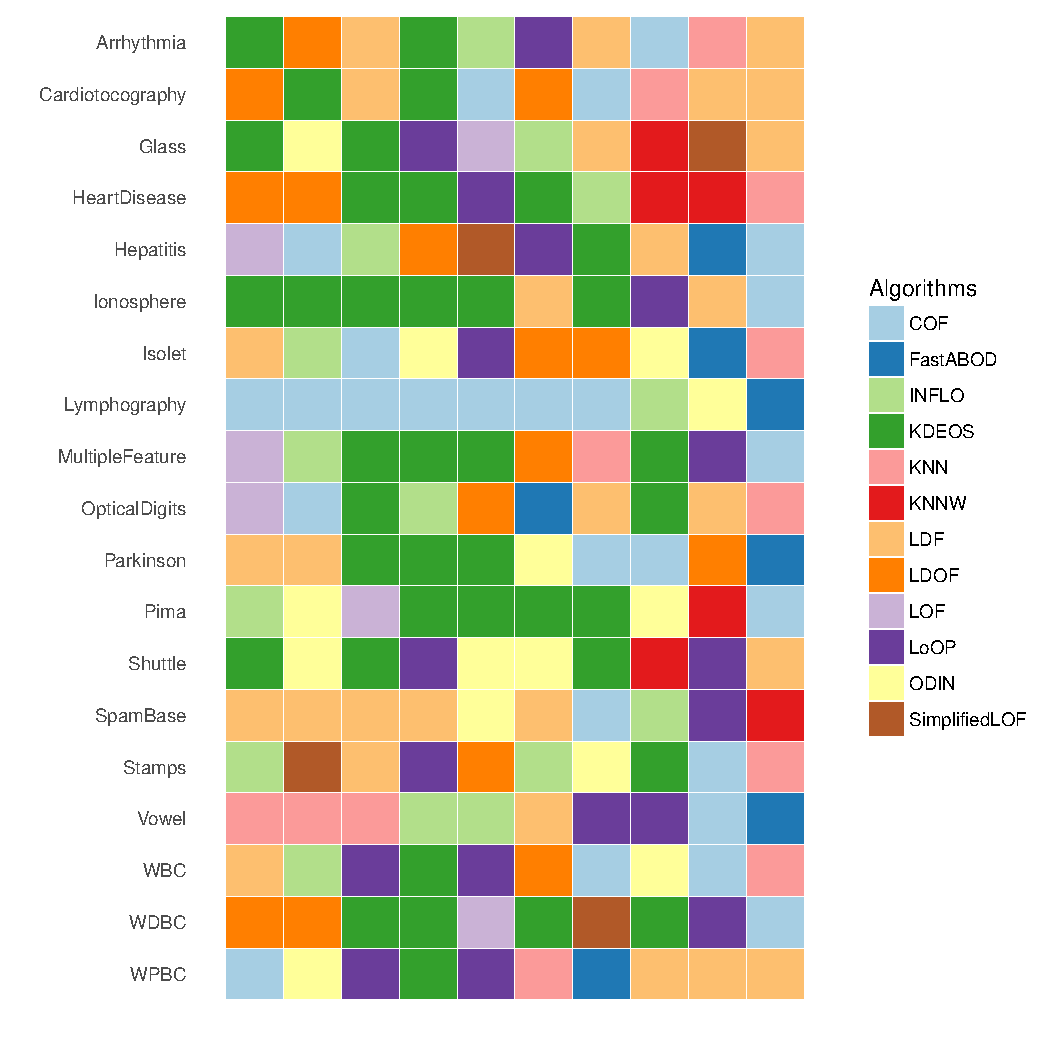
\includegraphics[width=0.65\textwidth]{figs/algorithms.pdf}
\captionsetup{justification=centering}
\caption{Distribution of the algorithms for the different solutions used in the experiments. Solutions are ordered in ascending order by ROC AUC: the first column is the worst solution and the last column is the best solution.}
\label{fig:algorithms}
\end{figure}

We perform two types of experiments. In the first, we assess the quality of the solutions produced by the outlier detection algorithms with respect to the 4 external measures and ext-IREOS. Then, we compute the Spearman correlation between the quality assessments of the solutions computed by ext-IREOS and quality assessments of the solution with respect to the ground truth using the external measures.

In the second type of experiment, we performed an experiment involving model selection. Using the quality assessments of the solutions computed by ext-IREOS we selected the best solution according to the ext-IREOS score, this solution is compared in terms of ROC AUC against the best, worst and expected (average) ROC AUC that can be obtained in the set of candidate solutions.

We evaluate ext-IREOS with $m_{cl}$ set to both extremes of the valid interval, in order to represent cases with ($m_{cl} = n$) and without ($m_{cl} = 1$) the optional mechanism for modeling clumps.
The number of discrete $\gamma$ values for the practical computation of the index was $n_{\gamma} = 100$ in all experiments.

\subsection{Results}

The results of the experiment of the Spearman correlation are presented in Fig. \ref{fig:correlation}. In the Fig. \ref{fig:correlation_1} and Fig. \ref{fig:correlation_n} are presented the correlation for $m_{cl} = 1$ and $m_{cl} = n$, respectively. Each line represents a dataset, each column the external measure correlated with ext-IREOS and the colors reflect the correlations: darker blue indicates higher correlations and darker red indicates lower correlations (Spearman correlation values are noted inside).  

Except for \textit{WBC} dataset, all the other datasets exhibit good correlations between the ext-IREOS and the external measures. Two correlated measures must be highlighted: the ROC AUC was the measure with the highest correlation with ext-IREOS, it was expected due to the fact that the ROC AUC be the only external measure that truly evaluates the whole ranking, as well as ext-IREOS. On the other hand, prec@$n$ was the measure with the lowest correlation with ext-IREOS, it was also expected because unlike the ROC AUC, the prec@$n$ is the only measure that considers only the observations ranked in the top-$n$.

\begin{figure}[ht!]
\center
\captionsetup{justification=centering}
\subfloat[ext-IREOS ($m_{cl} = 1$)]{\label{fig:correlation_1} 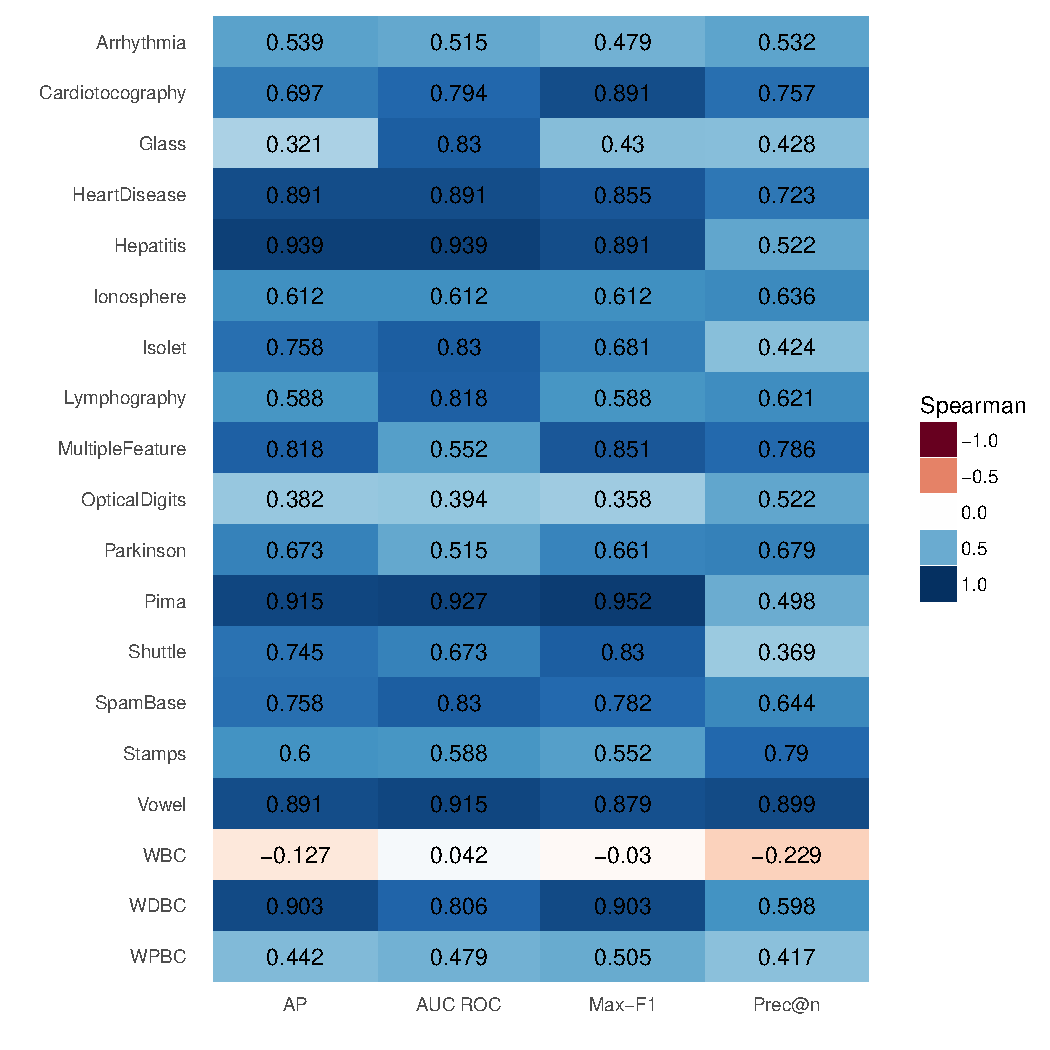
\includegraphics[width=0.5\textwidth]{figs/correlation_sep1.pdf}}
\subfloat[ext-IREOS ($m_{cl} = n$)]{\label{fig:correlation_n} 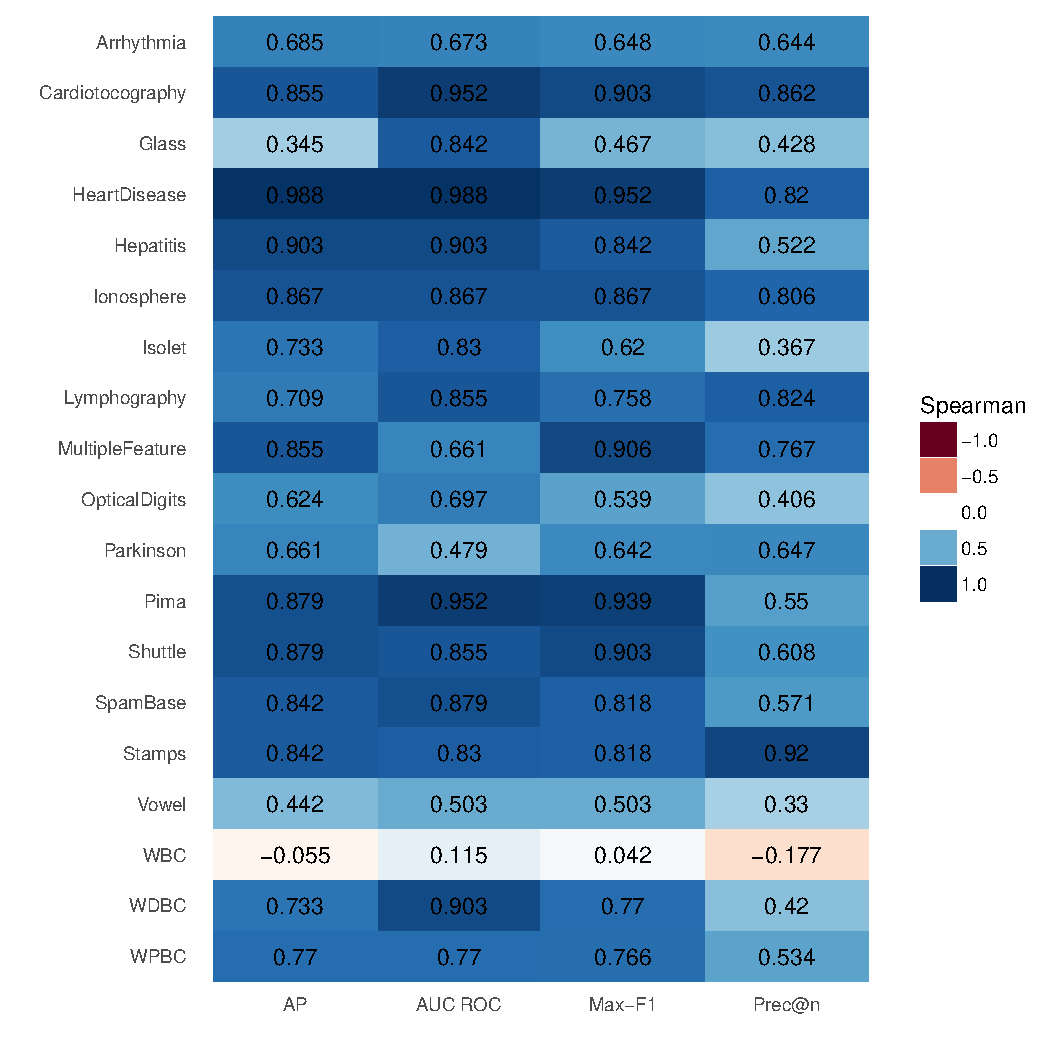
\includegraphics[width=0.5\textwidth]{figs/correlation_sepn.pdf}}
\caption{Spearman correlation of the ext-IREOS against external measures. \\ Colors reflect the correlations: darker blue indicates higher correlations and darker red indicates lower correlations}
\label{fig:correlation}
\end{figure}

The results of the model selection experiments are summarized in Table \ref{tab:model_selection}, showing ROC AUC for the worst, the expected (average), and the best cases among the candidates, along with ROC AUC for the solution selected as best according to ext-IREOS; for each selected solution, the table also indicates which algorithm produced this solution.

By using ext-IREOS with $m_{cl} = n$ one would select the most accurate solution according to the ground truth in 12 out of the 19 datasets. ext-IREOS with $m_{cl} = 1$ makes the best choice for 10 out of the 19. In the other cases, the choice is always close to the best possible selection according to the ground truth. For both, $m_{cl} = n$ and  $m_{cl} = 1$, the selected solution is among the top 3 best possible selection according to the ground truth in 18 out of the 19 datasets. In all cases, the solution selected is better than the expected value, which could not be guaranteed without any validation index. To get a better sense where the selected solutions are located within the distribution of the ROC AUC values for all candidate solutions, we also show box plots of the distributions for each dataset in Fig. \ref{fig:boxplot}. The positions of the solutions selected by ext-IREOS are indicated by special symbols in the plots.

\begin{table}[ht!]
\centering
\captionsetup{justification=centering}
\caption{Summarization of the ROC AUC values for all candidate solutions used in the experiments. Two last columns indicate the solutions selected by ext-IREOS for $m_{cl} = 1$ and $m_{cl} = n$ respectively}
\label{tab:model_selection}
\begin{tabular}{@{}llllllll@{}}
\toprule
\multicolumn{1}{l}{Dataset} & Min & Max & \multicolumn{1}{l}{Avg} & \multicolumn{2}{l}{ext-IREOS ($m_{cl} = 1$)} & \multicolumn{2}{l}{ext-IREOS($m_{cl} = n$)} \\ \midrule
\multicolumn{1}{l|}{Arrhythmia}        &  0.5003   &   0.9156  & \multicolumn{1}{l|}{0.7368}    &     0.8794     & \multicolumn{1}{l|}{KNN}         &         0.8794           &       KNN             \\
\multicolumn{1}{l|}{Cardiotocography}        &    0.513 &   0.8199  & \multicolumn{1}{l|}{0.6716}    &     0.7559     & \multicolumn{1}{l|}{KNN}         &     0.8199               &     LDF               \\
\multicolumn{1}{l|}{Glass}        &  0.4921   &  0.9035   & \multicolumn{1}{l|}{0.6987}    &     0.8585     & \multicolumn{1}{l|}{SimplifiedLOF}         &      0.9035              &        LDF            \\
\multicolumn{1}{l|}{Heart Disease}        &   0.3867  &  0.9695   & \multicolumn{1}{l|}{0.687}    &    0.8467      & \multicolumn{1}{l|}{KNNW}         &        0.9695            &      KNN              \\
\multicolumn{1}{l|}{Hepatitis}        &  0.0746   &  0.9602   & \multicolumn{1}{l|}{0.5219}    &     0.9602     & \multicolumn{1}{l|}{COF}         &           0.9602         &          COF          \\
\multicolumn{1}{l|}{Ionosphere}        &  0.5143   &  0.9603   & \multicolumn{1}{l|}{0.745}    &   0.8677       & \multicolumn{1}{l|}{LoOP}         &          0.8677          &        LoOP            \\
\multicolumn{1}{l|}{Isolet}        &  0.1962   &  1   & \multicolumn{1}{l|}{0.6077}    &     1     & \multicolumn{1}{l|}{KNN}         &            1        &               KNN     \\
\multicolumn{1}{l|}{Lymphography}        &   0.4131  &   1  & \multicolumn{1}{l|}{0.7117}    &     1     & \multicolumn{1}{l|}{FastABOD}         &              1      &          FastABOD          \\
\multicolumn{1}{l|}{Multiple Feature}        &  0.3613   &  0.9937   & \multicolumn{1}{l|}{0.6862}    &     0.7917     & \multicolumn{1}{l|}{KNN}         &       0.9937             &       COF             \\
\multicolumn{1}{l|}{Optical Digits}        &   0.222  &   0.9993  & \multicolumn{1}{l|}{0.6157}    &     0.9993     & \multicolumn{1}{l|}{KNN}         &            0.7477        &     LDF               \\
\multicolumn{1}{l|}{Parkinson}        &  0.4479   &   1  & \multicolumn{1}{l|}{0.7646}    &     1     & \multicolumn{1}{l|}{FastABOD}         &         1           &          FastABOD          \\
\multicolumn{1}{l|}{Pima}        &   0.4636   &   0.779  & \multicolumn{1}{l|}{ 0.6273}    &     0.7466     & \multicolumn{1}{l|}{KNNW}         &         0.7466           &     KNNW               \\
\multicolumn{1}{l|}{Shuttle}        &   0.4154  &   0.9922  & \multicolumn{1}{l|}{0.7085}    &     0.9313     & \multicolumn{1}{l|}{LoOP}         &        0.8701            &     KNNW               \\
\multicolumn{1}{l|}{Spam Base}        &  0.4626   &  0.7794  & \multicolumn{1}{l|}{0.6245}    &   0.7794       & \multicolumn{1}{l|}{KNNW}         &         0.7794           &        KNNW            \\
\multicolumn{1}{l|}{Stamps}        &  0.3797   &   0.9207  & \multicolumn{1}{l|}{0.6547}    &   0.9207       & \multicolumn{1}{l|}{KNN}         &         0.9207           &        KNN            \\
\multicolumn{1}{l|}{Vowel}        &  0.2233   &   1  & \multicolumn{1}{l|}{0.6142}    &       1   & \multicolumn{1}{l|}{FastABOD}         &            0.9156        &               COF     \\
\multicolumn{1}{l|}{WBC}        &   0.4385  &   0.9972  & \multicolumn{1}{l|}{0.7209}    &   0.9972       & \multicolumn{1}{l|}{KNN}         &        0.9972            &      KNN              \\
\multicolumn{1}{l|}{WDBC}        &   0.3415  &   1  & \multicolumn{1}{l|}{0.6893}    &      1    & \multicolumn{1}{l|}{COF}         &          1          &       COF             \\
\multicolumn{1}{l|}{WPBC}        &   0.4007  &  0.5829   & \multicolumn{1}{l|}{0.4929}    &      0.5432    & \multicolumn{1}{l|}{LDF}         &            0.5432        &       LDF             \\ \bottomrule
\end{tabular}
\end{table}

\begin{figure}[ht!]
\center
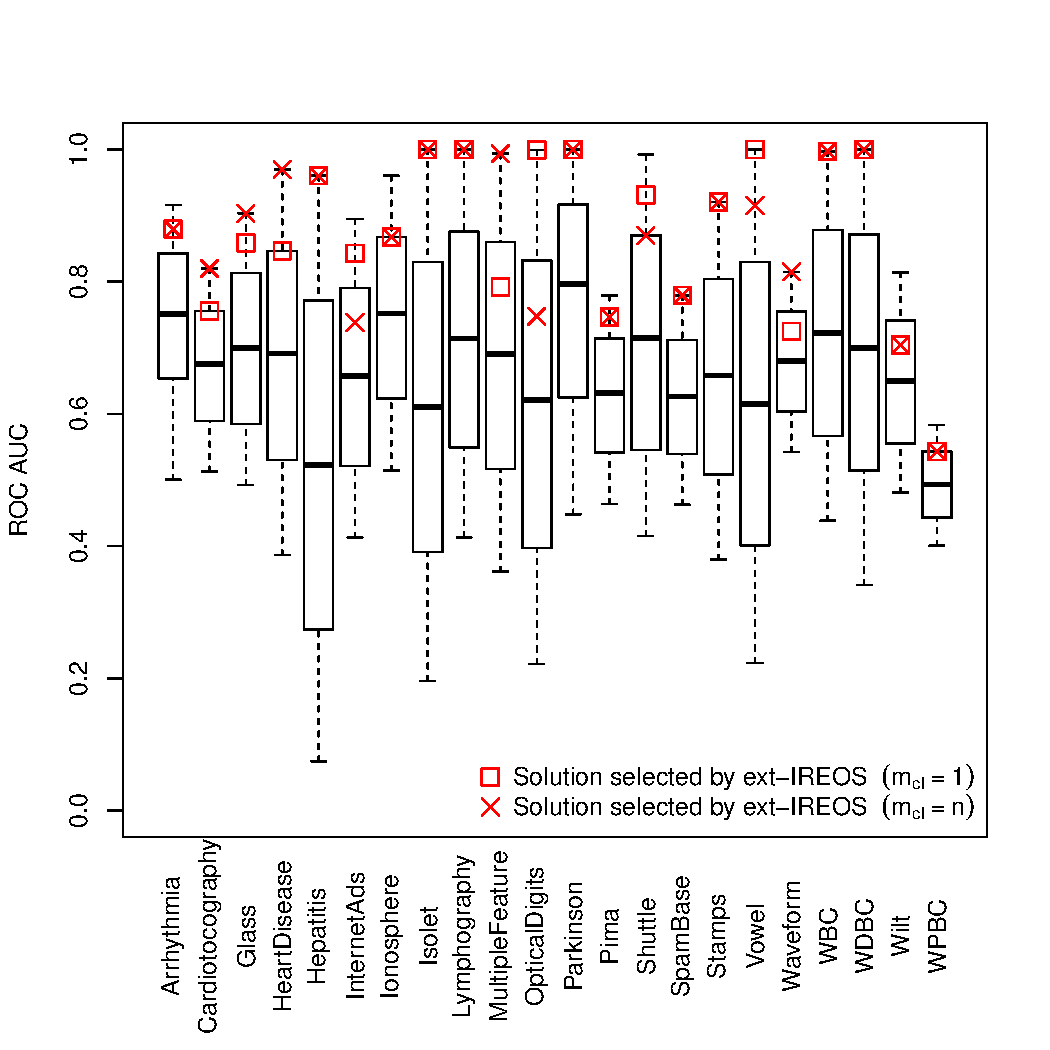
\includegraphics[width=\textwidth]{figs/boxplot.pdf}
\captionsetup{justification=centering}
\caption{Distribution of the ROC AUC values for all candidate solutions used in the experiments. The position of the solutions selected by ext-IREOS for $m_{cl} = 1$ and $m_{cl} = n$ are indicated by symbols of different shapes (encoding the two values of $m_{cl}$). Some symbols are superposed.}
\label{fig:boxplot}
\end{figure}

\newpage
